% !TeX root = ../main.tex
\documentclass[./../main.tex]{subfiles}

\begin{document}

\subsection{Mô hình ca sử dụng}

\subsubsection{Sơ đồ chính}

Hình \ref{fig:use_case_diagram} mô tả tác nhân và ca sử dụng chính của hệ thống.

\begin{figure}[h!]
	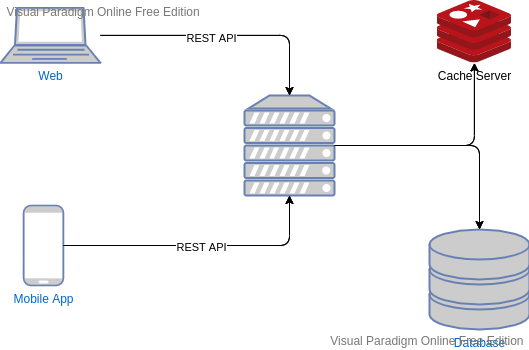
\includegraphics[width=\linewidth]{./images/image4.png}
	\caption{Mô hình ca sử dụng}
	\label{fig:use_case_diagram}
\end{figure}

\subsubsection{Tác nhân của hệ thống}

\begin{itemize}
	\item

	      \textbf{Người dùng} là người đã có tài khoản để truy cập vào hệ thống.

	\item

	      \textbf{Sinh viên} là người dùng hệ thống, sử dụng hệ thống để đăng ký
	      thực tập, nộp báo cáo và xem kết quả thực tập.

	\item

	      \textbf{Giảng viên} là người dùng hệ thống, sử dụng hệ thống để quản
	      lý và chấm điểm cho danh sách sinh viên đang hướng dẫn.

	\item

	      \textbf{Đối tác} là người dùng hệ thống, sử dụng hệ thống để quản lý
	      bài đăng tuyển dụng, danh sách yêu cầu thực tập và danh sách sinh viên
	      đang thực tập tại đơn vị.

	\item

	      \textbf{Quản trị viên Khoa} là người dùng hệ thống, sử dụng hệ thống
	      để quản lý danh sách các kỳ thực tập, danh sách sinh viên, đơn vị thực
	      tập, giảng viên theo từng kỳ và thông tin cá nhân của các đối tượng
	      đó.

	\item

	      \textbf{Quản trị viên} là người dùng hệ thống, sử dụng hệ thống để
	      quản lý danh sách các Khoa, danh sách lớp và quản lý tài khoản người
	      dùng hệ thống.

\end{itemize}

\subsection{Yêu cầu chức năng}

\hypertarget{ux111ux103ng-nhux1eadp-hux1ec7-thux1ed1ng}{%
	\subsubsection{Đăng nhập hệ
		thống}\label{ux111ux103ng-nhux1eadp-hux1ec7-thux1ed1ng}}

Người dùng cung cấp email và mật khẩu để truy cập vào hệ thống.

Ngoài đăng nhập bằng email và mật khẩu, người dùng có thể đăng nhập bằng Google.

\hypertarget{ux111ux1eb7t-lux1ea1i-mux1eadt-khux1ea9u}{%
	\subsubsection{Đặt lại mật
		khẩu}\label{ux111ux1eb7t-lux1ea1i-mux1eadt-khux1ea9u}}

Người dùng sử dụng chức năng này khi quên mật khẩu tài khoản. Hệ thống
sẽ yêu cầu người dùng nhập email VNU và gửi một đường link đặt lại mật
khẩu cho người dùng.

\hypertarget{ux111ux1ed5i-mux1eadt-khux1ea9u}{%
	\subsubsection{Đổi mật khẩu}\label{ux111ux1ed5i-mux1eadt-khux1ea9u}}

Người dùng có thể đổi mật khẩu.

\hypertarget{chux1ec9nh-sux1eeda-thuxf4ng-tin-cuxe1-nhuxe2n}{%
	\subsubsection{Chỉnh sửa thông tin cá
		nhân}\label{chux1ec9nh-sux1eeda-thuxf4ng-tin-cuxe1-nhuxe2n}}

Người dùng \textbf{sinh viên}, \textbf{giảng viên} và \textbf{đối tác}
có thể chỉnh sửa thông tin cá nhân của bản thân.

\hypertarget{xem-thuxf4ng-tin-buxe0i-ux111ux103ng}{%
	\subsubsection{Xem thông tin bài
		đăng}\label{xem-thuxf4ng-tin-buxe0i-ux111ux103ng}}

Người dùng \textbf{sinh viên} có thể xem thông tin cơ bản về bài đăng,
bao gồm:

\begin{itemize}
	\item Tiêu đề bài viết
	\item Thời gian đăng
	\item Tên công ty tuyển dụng
	\item Thông tin liên lạc của công ty
	\item Thông tin về vị trí, số lượng, thời hạn tuyển dụng
	\item Nội dung bài viết
\end{itemize}

\subsubsection{Xem quy chế thực tập}

Người dùng \textbf{sinh viên} có thể đọc về quy chế thực tập và hướng
dẫn sử dụng hệ thống.

\hypertarget{ux111ux103ng-kuxfd-thux1ef1c-tux1eadp-vux1edbi-cuxf4ng-ty-liuxean-kux1ebft}{%
	\subsubsection{Đăng ký thực tập với công ty liên
		kết}\label{ux111ux103ng-kuxfd-thux1ef1c-tux1eadp-vux1edbi-cuxf4ng-ty-liuxean-kux1ebft}}

Người dùng \textbf{sinh viên} đang trong thời gian thực tập chuyên ngành
có thể tìm kiếm và đăng ký thực tập với công ty liên kết. Nếu công ty
tìm kiếm không thuộc công ty liên kết, người dùng cần đăng ký thực tập
với công ty ngoài.

\hypertarget{ux111ux103ng-kuxfd-thux1ef1c-tux1eadp-vux1edbi-cuxf4ng-ty-ngouxe0i}{%
	\subsubsection{Đăng ký thực tập với công ty
		ngoài}\label{ux111ux103ng-kuxfd-thux1ef1c-tux1eadp-vux1edbi-cuxf4ng-ty-ngouxe0i}}

Người dùng \textbf{sinh viên} đang trong thời gian thực tập chuyên ngành
có thể tìm kiếm và yêu cầu đăng ký thực tập với công ty ngoài. Các yêu
cầu này cần được Khoa xét duyệt và có thể bị từ chối.

\begin{itemize}
	\item

	      Nếu công ty đã có trong cơ sở dữ liệu thì người dùng sinh viên có thể
	      gửi yêu cầu thực tập và đợi kết quả xét duyệt từ Khoa.

	\item

	      Nếu công ty chưa có trong cơ sở dữ liệu thì người dùng sinh viên phải
	      gửi thông tin công ty cho Khoa xét duyệt và đợi kết quả từ Khoa trước
	      khi gửi yêu cầu thực tập.

\end{itemize}

\hypertarget{ux111ux103ng-kuxfd-phux1ecfng-vux1ea5n-tux1eeb-buxe0i-ux111ux103ng}{%
	\subsubsection{Đăng ký phỏng vấn từ bài
		đăng}\label{ux111ux103ng-kuxfd-phux1ecfng-vux1ea5n-tux1eeb-buxe0i-ux111ux103ng}}

Người dùng \textbf{sinh viên} chưa đi thực tập tại đơn vị nào có thể
đăng ký phỏng vấn vào các công ty đang đăng bài tuyển dụng.

\hypertarget{xem-thuxf4ng-tin-thux1ef1c-tux1eadp}{%
	\subsubsection{Xem thông tin thực
		tập}\label{xem-thuxf4ng-tin-thux1ef1c-tux1eadp}}

Người dùng \textbf{sinh viên} có thể xem thông tin của mình trong kỳ
thực tập. Thông tin bao gồm:

\begin{itemize}
	\item

	      Công ty đã chọn

	\item

	      Thông tin của giảng viên hướng dẫn

	\item

	      Danh sách công ty đã đỗ và chưa đỗ phỏng vấn

\end{itemize}

\hypertarget{chux1ecdn-cuxf4ng-ty-ux111ux1ec3-thux1ef1c-tux1eadp}{%
	\subsubsection{Chọn công ty để thực
		tập}\label{chux1ecdn-cuxf4ng-ty-ux111ux1ec3-thux1ef1c-tux1eadp}}

Nếu đỗ phỏng vấn nhiều công ty, người dùng \textbf{sinh viên} bắt buộc
phải chọn một công ty để thực tập.

\hypertarget{nux1ed9p-buxe1o-cuxe1o-thux1ef1c-tux1eadp}{%
	\subsubsection{Nộp báo cáo thực
		tập}\label{nux1ed9p-buxe1o-cuxe1o-thux1ef1c-tux1eadp}}

Người dùng \textbf{sinh viên} có thể nộp báo cáo thực tập để được giảng
viên hướng dẫn nhận xét và chấm điểm.

\hypertarget{tux1ea3i-luxean-cv}{%
	\subsubsection{Tải lên CV}\label{tux1ea3i-luxean-cv}}

Người dùng \textbf{sinh viên} có thể tải lên CV. CV này sẽ có thể được
xem bởi công ty và giảng viên hướng dẫn trong quá trình chấp nhận và từ
chối yêu cầu thực tập.

\hypertarget{xem-thux1ed1ng-kuxea-dux1eef-liux1ec7u-truxean-hux1ec7-thux1ed1ng}{%
	\subsubsection{Xem thống kê dữ liệu trên hệ
		thống}\label{xem-thux1ed1ng-kuxea-dux1eef-liux1ec7u-truxean-hux1ec7-thux1ed1ng}}

Người dùng \textbf{giảng viên, đối tác, quản trị viên Khoa, quản trị
	viên} có thể xem thống kê dữ liệu trên hệ thống.

\hypertarget{xem-danh-suxe1ch-sinh-viuxean-ux111ang-hux1b0ux1edbng-dux1eabn}{%
	\subsubsection{Xem danh sách sinh viên đang hướng
		dẫn}\label{xem-danh-suxe1ch-sinh-viuxean-ux111ang-hux1b0ux1edbng-dux1eabn}}

Người dùng \textbf{giảng viên} có thể xem danh sách sinh viên đang hướng
dẫn thực tập và thông tin cá nhân của những sinh viên đó.

\hypertarget{xem-buxe1o-cuxe1o-thux1ef1c-tux1eadp-cux1ee7a-sinh-viuxean}{%
	\subsubsection{Xem báo cáo thực tập của sinh
		viên}\label{xem-buxe1o-cuxe1o-thux1ef1c-tux1eadp-cux1ee7a-sinh-viuxean}}

Người dùng \textbf{giảng viên} có thể xem và tải về báo cáo thực tập của
sinh viên mình đang hướng dẫn.

\hypertarget{chux1ea5m-ux111iux1ec3m-cho-sinh-viuxean}{%
	\subsubsection{Chấm điểm cho sinh
		viên}\label{chux1ea5m-ux111iux1ec3m-cho-sinh-viuxean}}

Người dùng \textbf{giảng viên} có thể bổ sung đầu điểm giữa kỳ và cuối
kỳ cho sinh viên mình đang hướng dẫn thông qua biểu mẫu nộp điểm. Hai
đầu điểm này sẽ được sử dụng để tính ra điểm tổng kết cuối cùng.

\subsubsection{Yêu cầu chức năng khác}

Ngoài các yêu cầu chức năng liệt kê ở trên, hệ thống cũng có các yêu cầu chức năng sau. Các yêu cầu này sẽ được mô tả kỹ hơn ở tài liệu của bạn Phạm Thị Dân.

\begin{itemize}
	\item Quản lý bài đăng (cho đối tác)
	\item Quản lý yêu cầu thực tập của sinh viên
	\item Quản lý sinh viên đang thực tập tại công ty
	\item Quản lý kỳ thực tập
	\item Quản lý danh sách sinh viên đang thực tập
	\item Quản lý danh sách đối tác trong kỳ thực tập
	\item Quản lý bài đăng của các đối tác trong kỳ thực tập
	\item Quản lý giảng viên hướng dẫn trong kỳ thực tập
	\item Quản lý danh sách sinh viên
	\item Quản lý danh sách đối tác
	\item Quản lý danh sách giảng viên
	\item Quản lý danh sách người dùng
	\item Quản lý danh sách khoa
	\item Quản lý danh sách lớp
\end{itemize}

\subsection{Yêu cầu phi chức năng}

Hệ thống backend cần đạt được những yêu cầu phi chức năng sau.

\hypertarget{ux111ux1ed9-tin-cux1eady}{%
	\subsubsection{Độ tin cậy}\label{ux111ux1ed9-tin-cux1eady}}

Hệ thống không bị sập do lỗi phần mềm. Thời gian uptime của server sẽ
phụ thuộc vào bên quản lý hạ tầng.

\hypertarget{hiux1ec7u-suux1ea5t}{%
	\subsubsection{Hiệu suất}\label{hiux1ec7u-suux1ea5t}}

Phần này mô tả các yêu cầu phi chức năng liên quan đến hiệu suất của hệ
thống.

Hệ thống cần có sức chứa như sau:

\begin{itemize}
	\item

	      Hỗ trợ tối thiểu 500 yêu cầu đồng thời

	\item

	      Hỗ trợ tối thiểu 30000 thành viên

\end{itemize}

Hệ thống cần phải thỏa mãn những yêu cầu sau:

\begin{itemize}
	\item

	      Hoàn thành 95\% yêu cầu trong thời gian dưới 2 giây.

	\item

	      Hoàn thành 99\% yêu cầu trong thời gian dưới 5 giây.

\end{itemize}

\hypertarget{tuxednh-bux1ea3o-mux1eadt}{%
	\subsubsection{Tính bảo mật}\label{tuxednh-bux1ea3o-mux1eadt}}

Hệ thống cần:

\begin{itemize}
	\item

	      Đưa ra phương pháp để tránh lỗ hổng bảo mật trên ứng dụng Web như đề
	      xuất của
	      \href{https://owasp.org/www-project-top-ten/}{\underline{OWASP}}.

	\item

	      Cài đặt tính năng logging mỗi khi có thay đổi được thực hiện trong cơ
	      sở dữ liệu (thêm kỳ thực tập, xóa kỳ thực tập, \ldots).

\end{itemize}

\hypertarget{bux1ea3o-truxec-vuxe0-lux1b0u-chuyux1ec3n}{%
	\subsubsection{Bảo trì và lưu
		chuyển}\label{bux1ea3o-truxec-vuxe0-lux1b0u-chuyux1ec3n}}

Hệ thống cần cung cấp bộ ca kiểm thử đơn vị, tích hợp và hệ thống để sau
này có thể dễ dàng bảo trì và nâng cấp phần mềm.

\end{document}